%!TEX root = ../dissertation.tex
\begin{savequote}[75mm]
Before anything else, preparation is the key to success.
\qauthor{Alexander Graham Bell}
\end{savequote}

\chapter{Preparation}
\section{A11Y Guide}
In preperation for the main deliverable a deeper level of knowledge in the
accessibility space was required. To gain this knowledge and inline with my
'Share Everything' approach it was decided that an 'Accessibility
training guide' would be produced here on referred to as 'A11Y guide'. The idea
being that in producing a guide for others, oneself would have to be
knowledgable enough to produce good content.

\subsection{Planning}
% TODO - Reference curve: http://www.wranx.com/ebbinghaus-and-the-forgetting-curve/

As researched by Ebbinghaus in 1885 the forgetting curve demonstrates the
amount of knowledge remembered after a period of time. see Fig.~\ref{fig:ebbinghaus}
Repeating or revising the learning unsuprisingly results in the knowledge
stored in memory for longer.

\begin{figure}
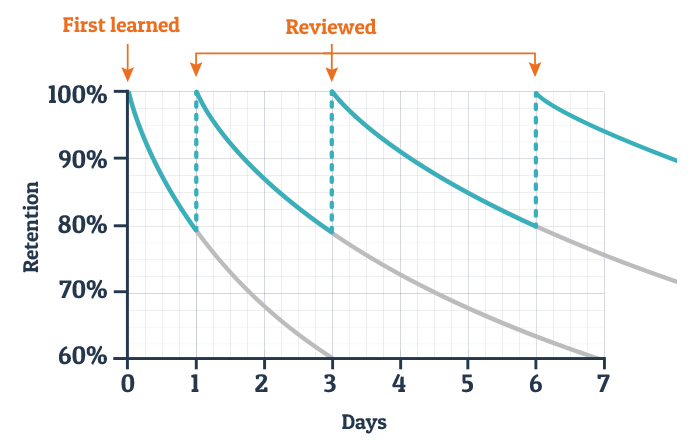
\includegraphics[width=\textwidth]{figures/ebbinghaus}
\caption[Short figure name.]{Ebbinghaus' famous forgetting curve
\label{fig:ebbinghaus}}
\end{figure}

With this in mind I plan to iteratively build the A11Y Guide so
that the knowledge will be reinforced. The steps for its production will be
as follows:
\begin{enumerate}
  \item Search for useful resources online (This will be first time learning)
  \item Score the identified resources with the assistive tools for a first hand
  experience along with other criteria (This second time repeating)
  \item Collate the resources under the correct header in a github project
  \item Setup continuous deployment scripts to ensure deploy on commit
  \item For each header create and document best practices (This third time
  repeating)
  \item Build a basic documentation website
  \item For each header create coded examples (This fourth time repeating)
\end{enumerate}

As explicitly stated there will be four loops of observing, reviewing and
applying the knowledge learned which should result in a peak knowledge level
when producing the tool.

\subsection{Building A11Y Guide Requirements}
In parallel to the above, for the guidance to have a greater impact it
needs to be current, relevant and available. This will require some additional
research into the current state of web frameworks and also the
requirements of Capgemini's teams. To do this I propose issuing a questionnaire to my
colleagues and using google trends to gain an understanding of the direction
of front end web development.

\subsubsection{Questionnaire}
Capgemini employees are

\subsubsection{Understanding industry movement}
\subsubsection{A11Y Guide Requirements}

\subsection{Gathering Knowledge}
\subsubsection{Method}
\subsubsection{Scoring}
\subsubsection{Outputs}

\subsection{Building the A11Y Guide}
\subsubsection{Iteration 1 - Create content using markdown}
\subsubsection{Iteration 2 - UI Design & Build site}
\subsubsection{Iteration 3 - Continue content}
\subsubsection{Iteration 4 - Recognise/Implement custom pages}
\subsubsection{Iteration 5 - Continue content}
\subsubsection{Iteration 6 - Generify}

\subsection{Extending the impact}
\subsubsection{Colour Contrast Tool}
\subsubsection{Markdown/React Documentation Framework}

\section{A11Y Analysis Tool}
\subsection{Requirements}
\subsection{Diagrams}
\subsection{Design}

\section{Additional }
% TODO - discuss Travis CI for report writing
% TODO - discuss Branching model
% TODO - discuss any Standards


Principally, this chapter should describe the work that was undertaken before
code was written, hardware built, theories worked on, or research studies
executed. It should show how the project proposal was further refined and
clarified, so that the implementation/research execution stage could go
smoothly rather than by trial and error. This part of the report is attempting to
prove that you went through a planning process before embarking on the
deliverable so among others it might include discussion of:

1. For software projects, a requirements analysis, HCI designs, architectural
and use-case diagrams, etc.
2. Any programming languages learnt, any complicated theories or algorithms
that required understanding
3. For research-based projects, the research approach (experimental design,
where applicable), including methods and tools that were used/applied. If the
research method involves the development of prototypic software to test a
concept, briefly describe the design, structure, and creation of this software.
Research methods should be described such that a third party could replicate
the study/experiment to validate the results.

This section should be answering the question “How did I plan to achieve the
deliverable?”
